\section{Lagrangian differentiation}
\label{sect:lagrange}

%\begin{figure}[!t] 
%  \centerline{
%              \includegraphics[width=0.9\textwidth,trim = 0mm 0mm 0mm 0mm,clip=]{images/l_diff_lin.eps}
%              }
%\caption[Lagrange difference technique simulation]{\emph{Top}: Simulated distance-time data with noise added. \emph{Middle}: Velocity-time data obtained using a three-point Lagrange difference technique. \emph{Bottom}: Acceleration-time data obtained using a three-point Lagrange difference technique. }
%\label{fig:l_diff_sim}
%\end{figure}

A more advanced numerical differentiation method is the three-point Lagrangian method used by the \textsc{deriv} routine in IDL. This method uses three adjacent points ($t-\Delta t$, $t$ and $t+\Delta t$) to fit a Lagrange polynomial function of the form
\begin{eqnarray}
P(x) &=& \frac{(x - t)(x - (t+\Delta t))}{((t-\Delta t) - t)((t-\Delta t)- (t+\Delta t))}y_{1} \nonumber \\
&+& \frac{(x - (t-\Delta t))(x - (t+\Delta t))}{(t - (t-\Delta t))(t - (t+\Delta t))}y_{2} \nonumber \\ 
&+& \frac{(x - (t-\Delta t))(x - t)}{((t+\Delta t) - (t-\Delta t))((t+\Delta t) - t))}y_{3}
\end{eqnarray}
to the three points, and hence find the derived value at a point numerically.

This method gives a more accurate indication of the numerically differentiated data as it does not assume a straight line in between points. In addition, the routine compensates for edge points, increasing the errors of the points. It also uses three points to find the numerical derivative, rather than two (c.f. centre, forward and reverse-difference techniques). The Lagrangian technique also smoothes the data-set, removing the spiky appearance that arises from use of the different Taylor series techniques.

\begin{deluxetable}{ccc}
\tablecolumns{3}
\tabletypesize{\small}
\tablewidth{0pt}
\centering
\tablecaption{Numerical differentiation errors \label{tbl:numdiff}}
\tablehead{
\colhead{Method} & \colhead{Kinematics} & \colhead{Error term}
}
\startdata
Forward diff. & Velocity &  $O(\Delta t) = \frac{r(t + 2\Delta t) - 2r(t + \Delta t) + r(t)}{2!\Delta t}$  \\
 & Acceleration & $O(\Delta t) = \frac{v(t + 2\Delta t) - 2v(t + \Delta t) + v(t)}{2!\Delta t}$   \\
Reverse diff. & Velocity &  $O(\Delta t) = \frac{r(t) - 2r(t - \Delta t) + r(t - 2\Delta t)}{2!\Delta t}$   \\
 & Acceleration & $O(\Delta t) = \frac{v(t) - 2v(t - \Delta t) + v(t - 2\Delta t)}{2!\Delta t}$   \\
Centre diff. & Velocity & $O(\Delta t^{2}) = \frac{r(t + 3\Delta t) - 3r(t + \Delta t) + 3r(t - \Delta t) - r(t - 3\Delta t)}{(3!)(8)\Delta t}$   \\
 & Acceleration & $O(\Delta t^{2}) = \frac{v(t + 3\Delta t) - 3v(t + \Delta t) + 3v(t - \Delta t) - v(t - 3\Delta t)}{(3!)(8)\Delta t}$   \\
Lagrangian & Velocity & $\sigma$  \\
 & Acceleration & $\sigma$  \\
\enddata
\end{deluxetable}

 The problems encountered in this work arise from the small data-sets available in the case of these disturbances. The small data-sets mean that there are only four or five points available of which three are needed to calculate the numerical derivative of each point. This makes the Lagrangian technique unsuitable for estimating the kinematics of these disturbances.

The three-point Lagrangian interpolation method used by IDL uses the standard deviation of the derivative calculated by the Lagrangian polynomial as the truncation error of the numerical derivative. This produces a consistent estimate of the mean truncation error that only varies with the end-points due to the increased uncertainty of these points.

Table~\ref{tbl:numdiff} shows the different estimates for the truncation error term for each numerical differencing technique. These truncation error estimates are given in terms of the original base function, the exception being for the Lagrangian technique, which takes the standard deviation of the Lagrange derivative at a point as the truncation error estimate at that point.


%Figure~\ref{fig:l_diff_sim} shows the three-point Lagrangian technique operating on the simulated data-set used for the forward, reverse and centre difference methods. This figure has the same scaling as Figures~\ref{fig:f_diff_sim} to \ref{fig:c_diff_sim} to show the difference in errors between the different methods. The Lagrangian technique has much lower errors than the forward or reverse difference methods, and also smaller errors than the centre difference method. The errors are comparable with the data itself, but are still much larger than is reasonable for accurate data analysis. The Lagrangian method also has a problem with the edges of numerically derived data, and often drags these points downwards. This can result in false conclusions being made about the derived data.
